\documentclass[10pt,showpacs,preprintnumbers,footinbib,amsmath,amssymb,aps,prl,twocolumn,groupedaddress,superscriptaddress,showkeys]{revtex4-1}
\usepackage{graphicx}
\usepackage{dcolumn}
\usepackage{bm}
\usepackage[colorlinks=true,urlcolor=blue,citecolor=blue]{hyperref}
\usepackage{color}
\usepackage{listings}

\newcommand{\deriv}[3][]{% \deriv[<order>]{<func>}{<var>}
	\ensuremath{ \frac{d^{#1} {#2}}{d {#3}^{#1}} } }

\begin{document}
\title{Project 1}
\author{Thomas Redpath}
\affiliation{Department of Physics, Michigan State University}
\begin{abstract}

We solve Poisson's equation numerically to examine the effects of tailoring a specialized algorithm on execution speed.
Our best algorithm requires $4n$ FLOPS where $n$ the dimensionality of the matrix. We also explore the onset of
round-off errors and loss of precision as dimensionality becomes large.

\end{abstract}
\maketitle

\section{Introduction}

Poisson's equation plays a central role in electromagnetism as it governs how the electric potential $\Phi$ arrises from a
localized charge distribution $\rho (\mathbf{r})$. Poisson's equation for spherically symmetric $\Phi$ and $\rho (\mathbf{r})$,
where the substitution $\Phi(r) = \phi(r)/r$ had been made:

\begin{equation*}
	\deriv[2]{\phi}{r}= -4\pi r\rho(r).
\end{equation*}
Re-writting this equation to let $f$ stand for the combination of the r.h.s. terms, letting $\phi \rightarrow u$ and
$r \rightarrow x$ and taking Dirichlet boundary conditions yields

\begin{equation*}
	-u''(x) = f(x), \hspace{0.5cm} x\in(0,1), \hspace{0.5cm} u(0) = u(1) = 0.
\end{equation*}
The solution is easily approximated by discretizing the interval $(0,1)$ and using a numerical definition of the second
derivative.

\section{Theory and algorithms}

\subsection{Discretizing Poisson's Equation}

The numerical definition of a second derivative is derived from taking a Taylor expansion of the function $u(x)$.
On a discretized interval, it may be expressed as

\begin{equation*}
	\deriv[2]{u}{x} _i \approx \frac{u_{i+1} + u_{i-1} - 2u_i}{h^2} + O(h^2)
\end{equation*}
where $h$ is the grid spacing and the subscripts index the grid points. With this notation, Poisson's equation may be
re-written as

\begin{equation*}
	- \frac{u_{i+1} + u_{i-1} - 2u_i}{h^2} = f_i
\end{equation*}
With this formulation, it is apparent that we can re-cast the discretized Poisson equation as a system of linear equations
for each grid point.

\begin{equation*}
	\mathbf{A} \mathbf{u} = h^2 \mathbf{f}
\end{equation*}
where $\mathbf{A}$ is a matrix with dimensionality given by the number of grid points $n$

\begin{equation*}
    \mathbf{A} = \begin{bmatrix}
                           2& -1& 0 &\dots   & \dots &0 \\
                           -1 & 2 & -1 &0 &\dots &\dots \\
                           0&-1 &2 & -1 & 0 & \dots \\
                           \dots & \dots   & \ddots &\ddots &\ddots & \dots \\
                           0&\dots & \dots & -1 &2& -1 \\
                           0&\dots & \dots & 0  &-1 & 2 \\
                      \end{bmatrix}
\end{equation*}
and $\mathbf{f}$ represents a column vector whose elements are given by the source function
evaluated at each of the grid points. For simplicity of notation, we will absorb the $h^2$ into the
column vector elements ($h^2 \mathbf{f} = \mathbf{b}$) so that the system of equations may
be written $\mathbf{Au} = \mathbf{b}$. By applying numerical methods to solve Poisson's
equation on a discretized grid with $n$ points, we are able to convert a second order differential
equation into a system of $n$ equations.

\subsection*{The General Algorithm}

The matrix $\mathbf{A}$ given above is a tridiagonal matrix with identical elements along
the main and ``1-off'' diagonals. Our first algorithm solves the system of equations for a general
tridiagonal matrix using Gaussian elimination to reduce the matrix to an upper diagonal matrix,
effectively solving for the last variable $u_n$, then backwards subtituting the result to solve
for the remaining unknowns.

\[
\begin{bmatrix}
	d_1 & a_1 & 0 & \dots & \dots & 0 \\
	c_1 & d_2 & a_2 & 0 & \dots & 0 \\
	0 & c_2 & d_3 & a_3 & 0 & \dots \\
	\vdots & & \ddots & \ddots & \ddots & \vdots \\
	\vdots & & & c_{n-2} & \ddots & a_{n-1}\\
	0 & & & & c_{n-1} & d_n \\
\end{bmatrix}
~
\begin{bmatrix}
	u_1\\
	u_2\\
	u_3\\
	u_4\\
	\vdots\\
	u_n\\
\end{bmatrix}
~
=
~
\begin{bmatrix}
	f_1\\
	f_2\\
	f_3\\
	f_4\\
	\vdots\\
	f_n\\
\end{bmatrix}
\]

The Gaussian elimination method uses the first row of the matrix to
eliminate elements below the main diagonal:
\begin{align*}
	\mathrm{R2} \rightarrow \tilde{R2}&:
	\begin{bmatrix}
		0 & (d_2 - a_1 c_1/d_1) & a_2 & 0 \dots & 0\\
	\end{bmatrix}
%%	\mathrm{R3} \rightarrow \tilde{R3}&:
%%	\begin{bmatrix}
%%		0 & 0 & d_3 - (c_2 / \tilde{d_2}) & a_3 - (c_2 / \tilde{d_2}) 0 \dots & 0 \\
%%	\end{bmatrix}
\end{align*}
The altered second row is subsequently used to eliminate below-diagonal terms in the row
below it until the solution for the $n^{\mathrm{th}}$ unknown is found. The
result may then be backsubstituted to solve for the rest of the unknowns.
Following this procedure, the diagonal elements are modified in the foward
substituion according to the formula

\begin{equation*}
	\tilde{d_i} = d_i - \frac{a_{i-1} c_{i-1}}{\tilde{d}_{i-1}}
\end{equation*}
and the right hand side elements are modified according to

\begin{equation*}
	\tilde{f_i} = f_i - \tilde{f}_{i-1} \frac{c_{i-1}}{\tilde{d}_{i-1}}
\end{equation*}

Reducing the matrix in this way gives

\begin{equation*}
	u_n = \frac{\tilde{f}_n}{\tilde{d}_n}
\end{equation*}
for the last unknown. The form for the backwards substition to determine the
rest of the unknowns it

\begin{equation*}
	u _i = \frac{\tilde{f}_i - a_i u_{i+1}}{\tilde{d}_i}
\end{equation*}

These three calculations must be made $n-1$ times to solve the problem. Considering
that there are three floating point operations (1 multiplication, 1 division,
1 subtraction) per calculation, we note that the compuatational requirements
for implementing this algorithm scale with the number of grid points $n$ as $9(n-1)$.

\subsection*{The Specialized Algorithm}

The procedure outlined above can be optimized by taking advantage of the form that
the matrix takes for the specific case of solving Poisson's equation
using the three-point formula. Since the tridiagonal matrix has 2 for all main
diagonal elements and $-1$ for all 1-off diagonal elements, we can make two
simplifications to the algorithm. First, we can precalculate the $\tilde{d}_i$
elements by noting that they are given by $(i+1)/i$. Second, we can substitute -1
in for the $a_i$ and $c_i$ elements. With these simplifications, the forward
substitution calculation reduces to

\begin{equation*}
	\tilde{f}_i = f_i + \frac{ \tilde{f}_{i-1}}{\tilde{d}_{i-1}}
\end{equation*}
and the backward substitution reduces to

\begin{equation*}
	u_i = \frac{ \tilde{f}_i + u_{i+1}} {\tilde{d}_i}
\end{equation*}
This streamlined algorithm requires 4 floating point operations per grid point.

\subsection*{LU Decomposition}

Another way to implement the Gaussian elimination is the LU Decomposition method.
This method involves decomposing our matrix $\mathbf{A}$ into a product of two
matrices: one with 1s on the main diagonal and nonzero elements only below the
main diagonal and a second matrix with nonzero elements only above the main
diagonal. This decomposition allows us to write our matrix equation in the form

\begin{equation*}
	\mathbf{A u} = \mathbf{LU u} = \mathbf{f}
\end{equation*}
which can be solved in two steps

\begin{equation*}
	\mathbf{U u} = \mathbf{y}; \hspace{0.5cm} \mathbf{L y} = \mathbf{f}
\end{equation*}

By construction the matrix $\mathbf{L}$ has an inverse (since its determinant
is equal to 1) that we can use to obtain

\begin{equation*}
	\mathbf{L}^{-1} \mathbf{u} = \mathbf{y}
\end{equation*}
The algorithms necessary to LU Decompose $\mathbf{A}$ are discussed in detail
in \citep{Morten} and \citep{Golub1996}. It can be shown that this process
requires on the order of $2/3 n^3$ floating point operations.

\section{Methods}

We implemented the general algorithm described above in a C++ program
that first dynamically allocates arrays to hold the main and ``1-off''
diagonal elements of the array, the R.H.S. vector, a vector to hold the
x positions of the grid points and an array to hold the analytic
result evaluated at each grid point. Next, we initiallize these arrays
then apply the forward and backward substitutions to populate an array
holding the numerical approximation to the solution at each grid point.

%% -------------------------- CODE LISTING -------------------------- %%

%% 
 \definecolor{mygreen}{rgb}{0,0.6,0}
 \definecolor{mygray}{rgb}{0.5,0.5,0.5}
 \definecolor{mymauve}{rgb}{0.58,0,0.82}

 \lstset{ %
   backgroundcolor=\color{white},   % choose the background color; you must add \usepackage{color} or \usepackage{xcolor}
   basicstyle=\footnotesize,        % the size of the fonts that are used for the code
   breakatwhitespace=false,         % sets if automatic breaks should only happen at whitespace
   breaklines=true,                 % sets automatic line breaking
   captionpos=b,                    % sets the caption-position to bottom
   commentstyle=\color{mygreen},    % comment style
   deletekeywords={...},            % if you want to delete keywords from the given language
   escapeinside={\%*}{*)},          % if you want to add LaTeX within your code
   extendedchars=true,              % lets you use non-ASCII characters; for 8-bits encodings only, does not work with UTF-8
   frame=single,	                   % adds a frame around the code
   keepspaces=true,                 % keeps spaces in text, useful for keeping indentation of code (possibly needs columns=flexible)
   keywordstyle=\color{blue},       % keyword style
   language=C++,                 % the language of the code
   otherkeywords={*,...},           % if you want to add more keywords to the set
   numbers=left,                    % where to put the line-numbers; possible values are (none, left, right)
   numbersep=5pt,                   % how far the line-numbers are from the code
   numberstyle=\tiny\color{mygray}, % the style that is used for the line-numbers
   rulecolor=\color{black},         % if not set, the frame-color may be changed on line-breaks within not-black text (e.g. comments (green here))
   showspaces=false,                % show spaces everywhere adding particular underscores; it overrides 'showstringspaces'
   showstringspaces=false,          % underline spaces within strings only
   showtabs=false,                  % show tabs within strings adding particular underscores
   stepnumber=2,                    % the step between two line-numbers. If it's 1, each line will be numbered
   stringstyle=\color{mymauve},     % string literal style
   tabsize=2,	                   % sets default tabsize to 2 spaces
   title=\lstname                   % show the filename of files included with \lstinputlisting; also try caption instead of title
 }

 \lstinputlisting[linerange={78-90}]{../src/proj1.cc}

As described in the previous section, the specialized algorithm
reduces the number of computations per grid point by taking
advantange of the form of tridiagonal matrix for this case. This
allows us to precalculate the values of the $\tilde{d}$ array
and simplify expressions involving the off-diagonal elements
(since these are all -1).

 \lstinputlisting[linerange={137-152}]{../src/proj1.cc}

The LU decomposition is implemented using a set of functions
provided by the instructor. The resulting arrays containing
the solution were written out to files where they could be
parsed and plotted using a simple Python script.


\section{Results and discussion}

\subsection{Execution time}

We applied each of the procedures discussed in the previous sections to solve
Poisson's equation. Table~\ref{tab:speedresults} compares the execution time
as a function of number of grid points for each algorithm. As expected, the
specialized algorithm which uses the minimal number of floating point
operations runs the fastest. The LU Decomposition method is the least efficient
since it sets up and manipulates a full $n \times n$ matrix. We also note
that trying to apply the LU Decomposition method with $n=1000$ results in a
segmentation fault.

\begin{table}
\centering
	\begin{tabular}{ c | c c c }
	 & \multicolumn{3}{c}{Time [$\mu$s]}\\
	$n$ & General & Specialized & LU Decomp\\
\hline
	$10^{1}$ & 2       & 2       & 10 \\
	$10^{2}$ & 7       & 5       & 3500 \\
	$10^{3}$ & 62      & 50      & 1700000\\
	$10^{4}$ & 600     & 555     & \\
	$10^{5}$ & 6100    & 5100    & \\
	$10^{6}$ & 32500   & 28300   & \\
	$10^{7}$ & 244000  & 205000  & \\
\hline
	\end{tabular}
	\caption{Summary of execution times for the algorithms used.
	We note that the execution time can vary from run to run due
	to variations in CPU load. The execution time also varies
	from platform to platform.}
	\label{tab:speedresults}
\end{table}

\subsection{Comparison to exact result}

For this project, we assume the source term $f(x) = 100 e ^{-10x}$.
This allows the solution to the differential equation to obtained as
$u(x) = 1 - (1 - e^{-10})x - e^{-10x}$. Direct substituion back into
the DE confirms that this is indeed the correct solution.

\begin{equation*}
	- u''(x) = - (-100 e^{-10x}) = 100 e^{-10x}
\end{equation*}

We can then compare the results of our numerical solutions directly
to the analytic results. FIG.~\ref{fig:compexact} plots the results
of the generalized algorithm compared to the exact solution. We can
see that the numerical estimation agrees well with the analytic
result once at least 100 grid points are used.

We can also compute the relative error between the numerical estimate
and the exact result

\begin{equation*}
	\epsilon = \log _{10} \left ( \left | \frac{v_i - u_i}{u_i}
	\right | \right )
\end{equation*}
where $v_i$ is the numerical estimate to the solution and $u_i$ is
the closed-form solution. There are two contributions to the error
of this estimation: (1) truncation error resulting from the way we
approximate the second derivative and (2) round-off error arising
from subtraction of nearly equal numbers. The form for total error
for the second derivative formula is derived in \citep{Mslides}.

\begin{equation*}
	|\epsilon | \leq \frac{f_0}{12} h^2 + \frac{2 \epsilon _M}{h^2} 
\end{equation*}
where $\epsilon _M$ is the limit set by the precision of a number's
machine representation (roughly $10^{-7}$ and $10^{-16}$ for single
and double precision respectively). The truncation error is
proportional to $h^2$ and decreases with decreasing step size. The
round-off error increases with decreasing step size and becomes the
dominating term for $h\sim 10^7$. This is shown in FIG.~\ref{fig:rerr}

\begin{figure*}
\centering
	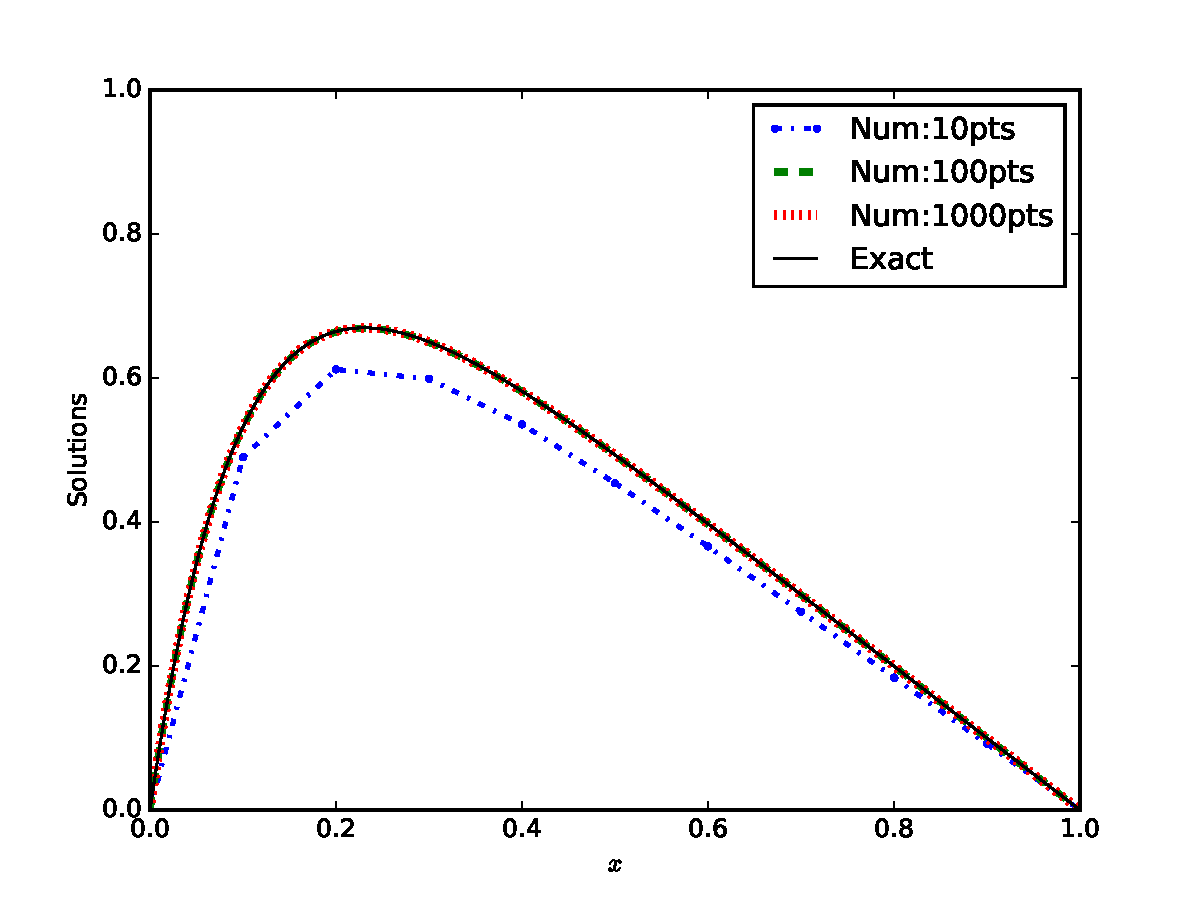
\includegraphics{figures/sols.pdf}
	\caption{A comparison of the results from the numerical solution
	(with various choices for the number of grid points) to the exact
	result. The blue curve plots the numerical result with 10 grid
	points, the green curve uses 100 grid points and the red curve
	uses 1000 grid points. The black curve plots the exact result.
	Good agreement with the exact result is obtained once 100 grid
	points are used.}
	\label{fig:compexact}
\end{figure*}

\begin{figure*}
\centering
	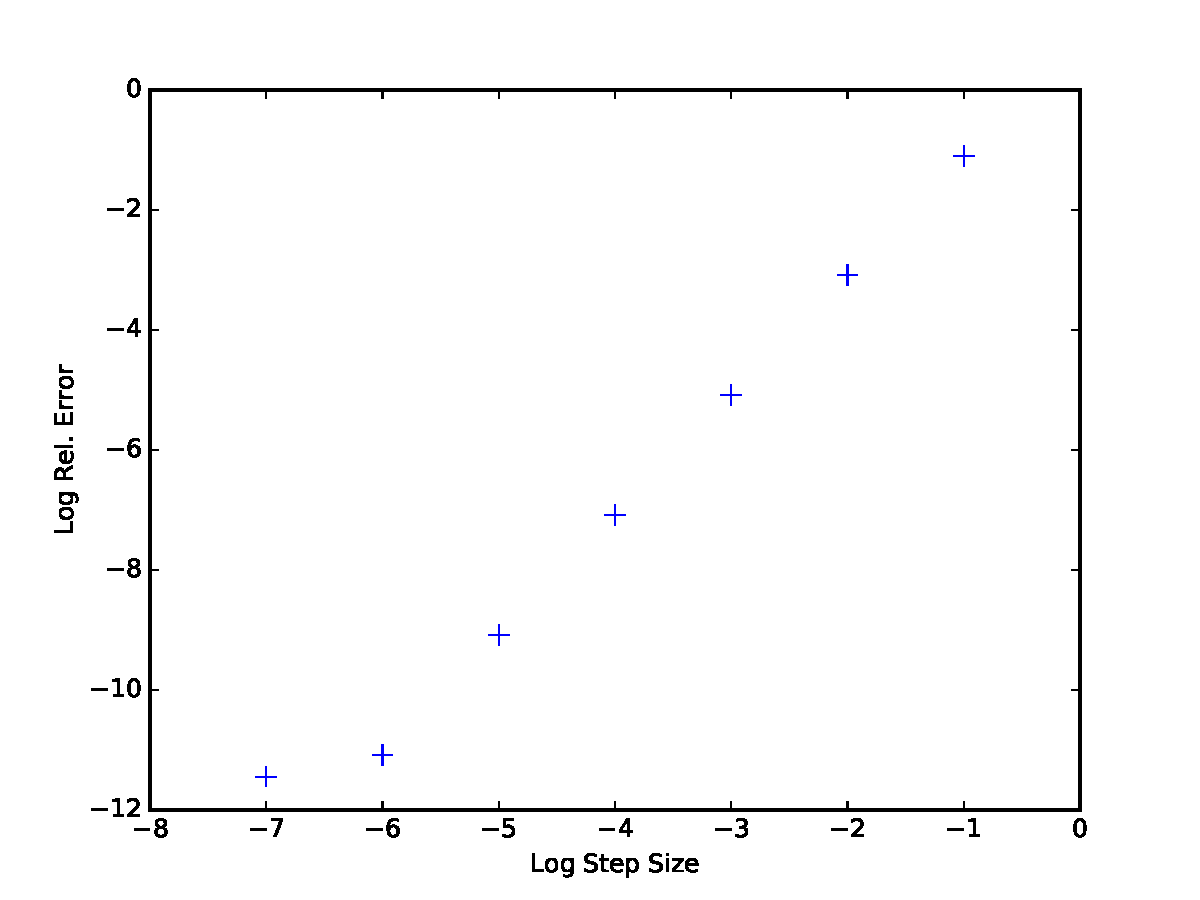
\includegraphics{figures/rerr.pdf}
	\caption{Log of the relative error vs. log of the step size.
	The slope of -2 for log step size between -6 and -1 corresponds
	to the decreasing error due to taking a smaller step size. This
	indicates that for these step sizes, the truncation error is
	the dominant term in the total error. This relationship disappears
	for log step size equal to -7 because the round-off error surpasses
	the truncation error as the dominant term in the total error.}
	\label{fig:rerr}
\end{figure*}



\section{Conclusions}

We have applied three different numerical algorithms to solve Poisson's
equation. As expected, the specialized algorithm runs the fastest since
it only stores and operates on the nonzero matrix elements while
the full LU decomposition is slowed down by cumbersome manipulations of
the full matrix. Additionally, we found that the round-off error begins
to dominate over the truncation error for step sizes $\sim h=10^7$.

\section{Appendix: Derivation of the Numerical Second Derivative Formula}

Consider a Taylor expansions for the function $f$ about some point $x$ from
above and below

\begin{align*}
	f(x+h) &= f(x) + h f'(x) + \frac{h^2}{2} f''(x) + \frac{h^3}{3!} f'''(x) +
	\frac{h^4}{4!} f^{(4)}\\
	f(x-h) &= f(x) - h f'(x) + \frac{h^2}{2} f''(x) - \frac{h^3}{3!} f'''(x) +
	\frac{h^4}{4!} f^{(4)}
\end{align*}
Adding these equations and solving for $f''(x)$ yields

\begin{equation*}
	f''(x) = \frac{f(x+h) - 2f(x) + (f(x-h)}{h^2} - \frac{h^2}{12}f^{(4)}
\end{equation*}
from this result, we see how the truncation error is proportional to $h^2$.


\begin{thebibliography}{99}
%\bibitem{miller2006} G.~A.~Miller, A.~K.~Opper, and E.~J.~Stephenson, Annu.~Rev.~Nucl.~Sci.~{\bf 56}, 253 (2006).
\bibitem{Morten} M. Hjorth-Jensen, Computational Physics Lecture Notes Fall 2015, August 2015.
\bibitem{Mslides} M. Hjorth-Jensen, Computational Physics Notes, compphysics.github.io
\bibitem{Golub1996} G. Golub, C. Van Loan, \textit{Matrix Computations} (John Hopkins University Press, 1996)
\end{thebibliography}

\end{document}
